\chapter{Algoritmos con base en caminatas cuánticas}
Empezando por el algoritmo de Shor para la factorización, los primeros algoritmos se basaban en la transformada de fourier para poder identificar un subgrupo escondido [Lomont 2004]. En los límites de este método se plantea la pregunta sobre otros posibles métodos eficientes, y una de las búsquedas se lleva a cabo en el área cuántica correspondiente a las  exitosas caminatas aleatorias clásicas.
En esta sección mencionamos algunos problemas de la computación para los cuales existe un algoritmo basado en una caminata cuántica que lo soluciona.\\

Iniciamos con el problema de atravesar la \textit{gráfica de árboles ligados} $G_n$, cuyo algoritmo fue el primero que incluyó una caminata cuántica con una mejora exponencial respecto de la clásica, en el marco del oráculo. En la sección anterior mostramos su dinámica, ahora cómo es posible aplicarla en un algoritmo. Esto nos sirve para presentar el concepto del \textit{oráculo}, en el que se basa el marco de comparación de eficiencia llamado \textit{complejidad de consultas}.\\

El algoritmo de Ambainis \cite{ambainis2007quantum} para resolver el problema de los elementos distintos en un conjunto sirve como base para implementación de otros algoritmos. Finalmente, el problema de la búsqueda espacial ha tenido diferentes soluciones. El esquema de búsqueda de Szegedy \cite{szegedy2004quantum} basado en la cuantización de la caminata, y las mejoras de Magníez et al. \cite{magniez2011search} son importantes. Un ejemplo de búsqueda espacial es sobre una base de datos física.\\

Los siguientes son problemas importantes solucionados con caminatas cuánticas sobre grafos adecuados:
\begin{itemize}{}
\setlength\itemsep{0.2em}
\item graph collision problem,
\item single source shortest path,
\item search on the grid(65-68[design]),
\item NAND true evaluation
\item forbidden subgraph propierty
\item tringle finding,
\item subset sum problem,
\item element distinctness problem,
\item group commutativity test,
\item matrix product verification,
\item Boolean matrix multiplication,
\item algebraic property test,
\end{itemize}{}

Los algoritmos se presentan con base en la estructura de \cite{shao}.
\section{Atravesar $G_n$ y $G_n'$}
\cite{childs2003exponential} presentaron el primer ejemplo de un algoritmo basado en caminatas cuánticas con ventaja exponencial. Usaron una modificación de $G_n$, llamada $G_n'$ (ver \ref{gr:Gn}). Conseguir tal ventaja sobre la gráfica $G_n$ no es posible ya que un algoritmo clásico logra el objetivo en un tiempo polinómico. $G_n'$, por su parte, no es resoluble en tiempo menor al exponencial. La modificación está en la unión de los dos árboles, en donde $G_n'$ tiene una distribución de aristas de la siguiente manera: vértice intermedio se conecta aleatoriamente con uno del otro costado de la mitad, el cual se conecta a su vez con otro del costado contrario, hasta conseguir una gráfica bipartita completa sobre esas dos columnas. \\

Los autores lo describen como un problema poco práctico pero capaz de demostrar el poder de las caminatas cuánticas. En el mismo trabajo presentaron la implementación del algoritmo como la simulación de un hamiltoniano conveniente.\\ 

El problema es el siguiente:\\

\textit{Dado un oráculo de la gŕafica $G_n$, y partiendo del vértice ENTRADA, ¿cuántos pasos cuesta llegar al vértica SALIDA?}\\

El oráculo de la gráfica da los nombres de los vértices vecinos al que le ingresamos. Describamos primero la solución En el marco del oráculo se tiene el siguiente algoritmo clásico óptimo, no basado en una caminata aleatoria, que toma $\mathcal{O}(t^2)$. Los vértices reciben nombres aleatoriamente. 

%\begin{center}
%    \begin{tabular}{l}
%    \hline \textbf{Algoritmo para cruzar $G_n$} \\\hline 
%    \textbf{1.} 
%    \\\hline
%    \end{tabular}{}
%\end{center}{}

\section{Búsqueda espacial}

El problema de búsqueda espacial es el siguiente:\\

\textit{Dada una gráfica, ¿cuántos pasos cuesta encontrar 1 o más elementos  marcados?}\\

Una búsqueda clásica corresponde a tomar aleatoriamente un vértice de la gráfica, verificar si es un elemento marcado, retornar el elemento y parar si lo encontró, o lanzar una moneda y moverse a lo largo de la arista etiquetada hasta llegar al nuevo vértice. El caminante repite el proceso aleatorio sin memoria del camino ni clave para encontrar el objetivo, que sólo alcanza cuando se para sobre el vértice marcado.\\

Un algoritmo de búsqueda típico se desarrolla en tres pasos: la etapa de preparación, la actualización y la verificación:
\begin{enumerate}
    \item $[$Preparar$]$ Acceder a algún estado de $\Gamma$, usualmente un estado aleatorio o uno de superposición uniforme en el caso cuántico,
    \item $[$Actualizar$]$ Llevar de un estado a otro estado con una caminata aleatoria (clásica o cuántica), y
    \item $[$Verificar$]$ verificar para saber si el estado actual está marcado.
\end{enumerate}

\begin{center}
    \begin{tabular}{|l|}
    \hline \textbf{Algoritmo de búsqueda clásico} por 1 paso de caminata aleatoria\\\hline 
    \textbf{1.} [Preparar] Obtener de $\Gamma$ un vértice $u$.\\
    \textbf{2.} Realizar lo siguiente $h=\mathcal{O}(1/(\epsilon \delta))$ número de veces, de acuerdo a la estimación [(5.11) Shao]:\\
    2.1. [Actualizar] Empezar desde $u$, simular una caminata aleatoria $P$ en $\Gamma$ en un paso.\\
    2.2 [Verificar] Si $u$ está marcado, retornar $u$ y  parar.\\
    \textbf{3.} Retornar "no ítem marcado"\\\hline
    \end{tabular}{}
\end{center}{}

\begin{center}
    \begin{tabular}{|l|}
    \hline \textbf{Algoritmo de búsqueda clásico} por multipasos de caminata aleatoria\\\hline 
    \textbf{1.} [Preparar] Obtener de $\Gamma$ un vértice $u$.\\
    \textbf{2.} Realizar lo siguiente $h(\pi^T,\mathcal{M})=\mathcal{O}(1/(\epsilon ))$ número de veces (que es el \textit{hitting time} promedio\\ desde la distribución estacionaria en $\Gamma$:\\
    2.2. [Actualizar] Empezar desde $u$, simular una caminata aleatoria $P$ en $\Gamma$ durante $T_{\text{mix}}=\mathcal{O}(1/\delta)$\\ pasos (hasta alcanzar la distribución estacionaria $\pi^T$).\\
    2.1 [Verificar] Si $u$ está marcado, retornar $u$ y  parar. \\
    \textbf{3.} Retornar "no ítem marcado"\\\hline
    \end{tabular}{}
\end{center}{}

\section{Algoritmos de búsqueda sobre grafos  finitos}
La idea de [Benioff, 2002] fue pionera en la  búsqueda espacial asociando a una región finita del espacio un grafo sobre cuyos vértices se para un \textit{robot cuántico}, y sobre cuyas aristas camina. Presentamos los casos cuánticos de la red finita en 2D con condiciones de frontera periódicos (que es un \textit{toro}) y el hipercubo que usan los resultados encontrados arriba.\\

La idea consiste en usar el operador de difusión de Grover $\hat{R}=2\sum_{v\in \mathcal{M}}\ket{v}\bra{v}-I$ en cada iteración (ver apéndice (\ref{sec:Grover})), intercalado con la caminata usual $\hat{U}$. Por el método de \textit{descomposición espectral} mostramos que tras un tiempo óptimo, la probabilidad de éxito es significativa.\\

Evaluamos en general el caso en que hay un solo elemento marcado, dado que para muchos elementos marcados, el resultado depende altamente de su distribución sobre el grafo. Llamando $0$ al vértice marcado, $\hat{R}=2\ket{0}\ket{0}-I$.\\

El operador de búsqueda es $\hat{U'}=\hat{U}\hat{R}$. Sean los autovalores $\{e^{i\lambda_1},\dots, e^{i\lambda_k}\}$ de $\hat{U'}$. Se puede mostrar que para tiempos grandes la búsqueda está determinada principalmente por dos autovalores de $\hat{U}'$, el de argumento que es el menor positivo, $\lambda$, y el de argumento que es el mayor negativo, $\lambda'$. (Ver gráfica \ref{gr:EspectroBusqueda}). Los respectivos autovectores son $\ket{\lambda}$ y $\ket{\lambda'}$. Lo anterior nos permite escribir para tiempos grandes:
\begin{figure}[ht]
\centering
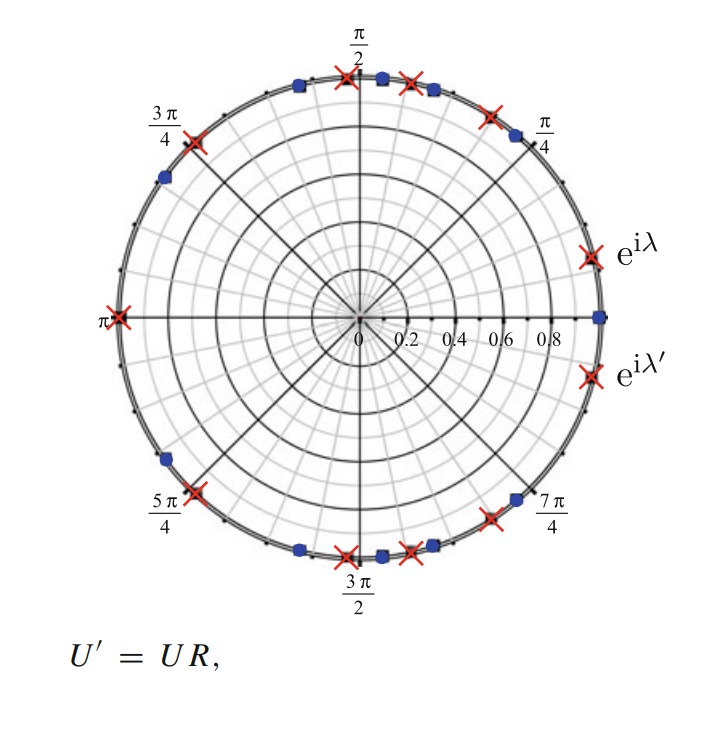
\includegraphics[width=0.5\textwidth]{Kap5/SpatialSearchUprimePortugal.png}
\caption{Autovalores de $\hat{U}$ y $\hat{U'}$. Para $t$ muy grandes $\lambda$ y $\lambda'$ tienden a 1, y son los únicos relevantes para la dinámica.
\cite{portugal2013quantum}}
\label{gr:EspectroBusqueda}
\end{figure}
\begin{equation}
    \hat{U}^t=e^{i\lambda t}\ket{\lambda}\bra{\lambda}+e^{i\lambda't}\ket{ \lambda'}\bra{\lambda'}+\hat{U}_{\text{pequeño}}^t
\end{equation}{}
La probabilidad de hallar $0$ en $t$ es $p(t)=|\braket{0|\hat{U}^t|\psi(0)}|^2$, 

\begin{equation}
    p(t)=|e^{i\lambda t}\braket{0|\lambda}\braket{\lambda|\psi(0)}+e^{i\lambda't}\braket{0|\lambda'}\braket{\lambda'|\psi(0)}+\epsilon|^2
    \label{ec:ProbEigenphaseDeco}\,\qquad\text{donde}\,\,\epsilon=\braket{0|\hat{U}^t_{\text{peq}}|\psi(0)}.
\end{equation}
$\hat{U}_{\text{peq}}$ actúa no trivialmente sobre el subespacio ortogonal al generado por los otros dos, $\{\ket{\lambda},\ket{\lambda'}\}^{\perp}$, pero $\lim_{t\xrightarrow{}\infty}\epsilon=0$.\\

El objetivo se cumple al encontrar $\lambda$, $\lambda'$, $\braket{0|\lambda}$, $\braket{0|\lambda'}$, y $\braket{\lambda|\psi(0)}$, $\braket{\lambda'|\psi(0)}$. En la estrategia de descomposición espectral, el primer paso es \textit{asumir} la descomposición de $\hat
{U}$: $\hat{U}\ket{\psi_k}=e^{i\phi_k}\ket{\psi_k}$.\\

Encontramos $\lambda$ resolviendo $A-B\lambda$-C$\lambda^2$=$\mathcal{O}(\lambda^3)$, con
\begin{align}
    A&=2\sum_{\phi_k=0}|\braket{0|\psi_k}|^2,\\
    B&=\sum_{\phi_k\neq0}\dfrac{|\braket{0|\psi_k}|^2\sin{\phi_k}}{1-\cos\phi_k},\\
    C&=\sum_{\phi_k\neq0}\dfrac{|\braket{0|\psi_k}|^2}{1-\cos\phi_k}.\\
\end{align}
Además,
\begin{align}
    \braket{0|\lambda}&=\dfrac{|\lambda|}{\sqrt{2}\sqrt{A+C\lambda ^2}}+\mathcal{O}(\lambda),\,\,\text{y}\\
    \braket{\psi(0)|\lambda}&=\braket{\psi(0)|0}\braket{0|\lambda}\Big(1+\frac{i\sin\lambda}{1-\cos\lambda}\Big)
\end{align}
Se puede demostrar que existe uno y sólo un autovalor $\lambda$. Si los autovalores de $\hat{U}$ vienen en pares complejos conjugados $e^{i\phi_k}$, y $e^{-i\phi_k}$, $B=0$, pues contiene $\sin\phi_k$ que es antisimétrica. En tal caso:

\begin{align}
    \lambda&=-\lambda'=\sqrt{\frac{A}{C}},\\
    \braket{0|\lambda}&=\braket{0|\lambda'}=\frac{1}{2\sqrt{C}},\\
    \braket{\psi(0)|\lambda}&=\braket{\psi(0)|0}\Big( \frac{1}{2\sqrt{C}}+\frac{i}{\sqrt{A}}\Big).
\end{align}
La probabilidad (\ref{ec:ProbEigenphaseDeco}):
\begin{equation}
    p(t)=\frac{|\braket{\psi(0)|0}|^2}{AC}\sin^2\lambda t
\end{equation}
de lo cual se tiene que $t_{\text{opt}}=\lfloor\frac{\pi}{2\lambda}\rfloor$, y $p_{\text{success}}(t)=\dfrac{|\braket{\psi(0)|0}|^2}{AC}$

\subsection{Gráfica 2D finita}
\begin{align}
    t_{\text{opt}}&=\lfloor\frac{\pi \sqrt{C}\sqrt{N\ln N}}{2\sqrt{2}}\rfloor\\
    p_{\text{exito}}&=\frac{1}{2C\ln N}+\mathcal{O}^{-N}
\end{align}
$\hat{U'}$ se puede expresar como $\hat{U'}=\hat{S}\hat{C'}$, que es una caminata cuántica en el modelo de moneda con dos particularidades: $\hat{S}$ es una moneda \textit{flip-flop}, que opera trasladando, y además cambia el estado de moneda al valor contrario. Por su parte, $\hat{C'}$ es una moneda inhomogenea dependiente de la posición.
\subsection{Hipercubo}

\begin{align}
    t_{\text{opt}}&=\lfloor\frac{\pi \sqrt{CN}}{4}\rfloor\\
    p_{\text{success}}&=\frac{1}{C}+\mathcal{N^{-1}}.
\end{align}
Esta búsqueda sobre el hipercubo basada en una caminata cuántica iguala la cota inferior del algoritmo de Grover.
Esta búsqeuda también se puede expresar como $\hat{U'}=\hat{S}\hat{C'}$.\\
\cite{shenvi2003quantum} \cite{ambainis2003quantum} Ambainis, 2003.
\begin{center}
    \begin{tabular}{|l|}
    \hline \textbf{Búsqueda en un hipercubo} \\\hline 
    \textbf{1.} [Preparar] Preparar el estado inicial $\ket{\psi}$:\\ $\ket{\psi}=\dfrac{1}{\sqrt{Nn}}\sum_{x,i}\ket{x}\ket{i}$\\
    \textbf{2.} Realizar lo siguiente $\mathcal{O}(\sqrt{N})$ número de veces:\\
    2.1. [Verificar y lanzar la moneda] Si $x$ no está marcado aplicar $\hat{R}$ al registro $\ket{i}$,\\
    sino aplicar $-I$ al registro $\ket{i}$\\
    2.2. [Actualizar] Aplicar $S:\ket{x}\ket{i}\xrightarrow{}\ket{\text{flip}(x,i)}\ket{i}$\\
    \textbf{3.} Medir el estado final del primero registro $\ket{x}$.\\\hline
    \end{tabular}{}
\end{center}{}



Trabajos posteriores modifican su método mejorando la eficiencia [Tulsi], [Ambainis]

\section{Otros marcos de búsqueda espacial}
\cite{magniez2011search} Magniez, 2011,
\cite{szegedy2004quantum} Szegedy presented a speed up for markov chains based algorithms. \\
Este es un ejemplo, \\
Loke, Wang\\

\begin{center}
    \begin{tabular}{l}
    \hline \textbf{Algoritmo de Szegedy} para detectar \textbf{si $|\mathcal{M}|=0$}\\\hline 
    \textbf{1.} Preparar el estado inicial $\ket{\pi}$:\\
    $\ket{\pi}=$\\
    \textbf{2.} Aplicar $\mathcal{O}(\sqrt{h})$ número de veces la siguiente caminata:\\
    $[$Chequeo y actualización simultáneas$]$ $W(P_M)$\\
    \textbf{3.} Construir el siguiente estado:\\
    $\frac{1}{2}\ket{0}(\ket{\pi}+(W(P_M))^t\ket{\pi})+\frac{1}{2}\ket{1}(\ket{\pi}-(W(P_M))^t\ket{\pi})$\\
    \textbf{4.} Medir el estado final en el registro de control.\\\hline
    \end{tabular}{}
\end{center}{}

Una aplicación interesante de estas caminatas se da en la memoria \textit{ECM} de un agente de aprendizaje por refuerzo llamado \textit{PS-agent} o agente de simulación proyectiva \cite{briegel2012projective}. Un agente de esta clase toma decisiones sobre sus acciones de acuerdo a la información que percibe del ambiente, bajo un marco llamado procesos de decisión de Markov. La ECM es un grafo dirigido en el cual los vértices son los posibles estados y acciones, algunos de los cuales se conectan por aristas que pueden contener refuerzos positivos o negativos, que generan preferencias sobre los caminos, es decir, cambios en las parejas estado-acción, que finalmente conduce al agente al aprendizaje de alguna conducta. 
[Paparo et al, 2014]  presenta una modificación del protocolo sobre el proceso de decisión del agente, basado en las caminatas cuánticas en el marco de Szegedy, y demuestra que efectivamente la velocidad del proceso mejora cuadráticamente como se espera, y además demuestra que el las características del aprendizaje del agente bajo ambos protocolos es el mismo (que es mensurable en las probabilidades de las acciones que generan). Esto es importante porque las características prácticas y exitosas del aprendizaje del agente no cambian. Un cambio en la demora de la decisión puede ser determinante en ambientes que cambian en tiempos del mismo orden de magnitud.


\begin{center}
    \begin{tabular}{l}
    \hline \textbf{Marco de caminata cuántica MNRS} \\\hline 
    \textbf{1.} Preparar el estado inicial $\ket{\pi}$:\\
    $\ket{\pi}=\sum_{u\in G}\sqrt{\pi_u}\ket{u}\ket{p_u}=\sqrt{\sum_{u\in M}\pi_u}\ket{\pi_{\text{good}}}+\sqrt{\sum_{u\not\in M}\pi_u}\ket{\pi_{\text{good}}}$\\
    \textbf{2.} Realizar lo siguiente $\mathcal{O}(1/\sqrt{\epsilon})$  número de veces:\\
    2.1. $[$Chequear$]$ Hacer la reflexión $R_{\ket{\pi_{\text{bad}}}}$ con respecto a $\ket{\pi_{bad}}$\\
    2.2. $[$Actualizar$]$ Hacer la reflexión $R_{\pi}$ con respecto a $\ket{\pi}$.\\
    \textbf{3.} Medir el estado final.\\\hline
    \end{tabular}{}
\end{center}{}
\begin{table}[h]
    \centering
    \begin{tabular}{|c|c|c|}
    \hline  
    Algoritmo & Costo para el caso $|\mathcal{M}|=1$ & Costo para el caso $\mathcal{M}>1$ \\\hline\hline
    Szegedy\cite{szegedy2004quantum} (2004)& $\sqrt{\frac{h}{N}}(S+\sqrt{h}(U+C))$ & $-$ \\\hline   
    MNRS (2011)&$S+\frac{1}{\sqrt{\epsilon}}(\frac{1}{\sqrt{\delta}}U+C)$ & $S+\frac{1}{\sqrt{\epsilon}}(\frac{1}{\sqrt{\epsilon}}U+C)$ \\\hline
    Magniez, et al (2012) & $S+\sqrt{h}(U+C)$ & $-$\\\hline
    Krovi, et al. (2016)& $S+\sqrt{h}(U+C)$&$S+\sqrt{h^+}(U+C)$
    \\\hline
    Dohotaru and Hoyer (2017)&$S+\sqrt{h}U+\frac{1}{\sqrt{\epsilon}}C$&$S+\sqrt{h^+}(U+C)$\\\hline
    \end{tabular}
    \caption{\cite{shao}}
    \label{AlgoritmosBusqueda}
\end{table}{}
